\chapter{Основы информационной безопасности} \label{chapt1}%
\textbf{Мета роботи:~}%
Изучение способов и основных концепций ИБ.
\section{Теоретические ведомости} \label{sect1_a}
%
\subsection{Основные понятия информационной безопасности}

Обеспечение защиты информации волновало человечество всегда. В процессе
эволюции цивилизации менялись виды информации, для её защиты применялись
различные методы и средства.

Процесс развития средств и методов защиты информации можно разделить на три
относительно самостоятельных периода:
\begin{figure}[ht]
  \centering
  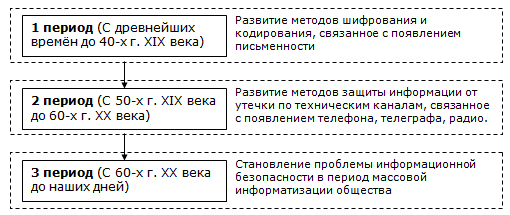
\includegraphics[width=\linewidth]{pr1_1}
  \caption{Периоды развития}\label{pr1_1}
\end{figure}

Наблюдаемые в последние годы тенденции в развитии информационных технологий
могут уже в недалеком будущем привести к появлению качественно новых
(информационных) форм борьбы, в том числе и на межгосударственном уровне,
которые могут принимать форму информационной войны, а сама информационная
война станет одним из основных инструментов внешней политики, включая защиту
государственных интересов и реализацию любых форм агрессии. Это является
одной из причин, почему полезно ознакомиться с основными принципами
обеспечения ИБ в ведущих зарубежных странах.

Прежде чем говорить об обеспечении безопасности персональных данных,
необходимо определить, что же такое информационная безопасность. Термин
<<информационная безопасность>> может иметь различный смысл и трактовку в
зависимости от контекста. В данном пособии под информационной безопасностью
мы будем понимать защищённость информации и поддерживающей инфраструктуры от
случайных или преднамеренных воздействий естественного или искусственного
характера, которые могут нанести неприемлемый ущерб субъектам информационных
отношений, в том числе владельцам и пользователям информации и поддерживающей
инфраструктуры.\href{https://www.intuit.ru/studies/courses/697/553/literature#literature.1}{\todo{[1]}}

\textbf{Информационная безопасность}~---~это защищённость информации и
поддерживающей её инфраструктуры от случайных или преднамеренных воздействий
естественного или искусственного характера, которые могут нанести ущерб
владельцам или пользователям информации.

В ряде случаев понятие <<информационная безопасность>> подменяется термином
<<компьютерная безопасность>>. В этом случае информационная безопасность
рассматривается очень узко, поскольку компьютеры только одна из составляющих
информационных систем. Несмотря на это, в рамках изучаемого курса основное
внимание будет уделяться изучению вопросов, связанных с обеспечением режима
информационной безопасности применительно к вычислительным системам, в
которых информация хранится, обрабатывается и передаётся с помощью
компьютеров. Согласно определению, компьютерная безопасность зависит не
только от компьютеров, но и от поддерживающей инфраструктуры, к которой можно
отнести системы электроснабжения, жизнеобеспечения, вентиляции, средства
коммуникаций, а также обслуживающий персонал.


\subsection{Составляющие информационной безопасности}%
Обеспечение информационной безопасности в большинстве случаев связано с
комплексным решением трёх задач:
\begin{Notes}
  \item \textbf{Конфиденциальность} – состояние информации, при котором
      доступ к ней осуществляют только субъекты, имеющие на него право.
  \item \textbf{Целостность} – состояние информации, при котором
      отсутствует любое её изменение либо изменение осуществляется только
      преднамеренно субъектами, имеющими на него право;
  \item \textbf{Доступность} – состояние информации, при котором субъекты,
      имеющие право доступа, могут реализовывать его беспрепятственно.
\end{Notes}

\textbf{Угрозы информационной безопасности}~---~совокупность условий и
факторов, создающих потенциальную или реально существующую опасность
нарушения безопасности информации.
\href{https://www.intuit.ru/studies/courses/697/553/literature#literature.1}{[2,3]}

\textbf{Атака}~---~это попытка реализации угрозы. Кто предпринимает такую
попытку, называется \textbf{злоумышленником}. Потенциальные злоумышленники
называются \textbf{источниками угрозы}.

Угроза является следствием наличия уязвимых мест или уязвимости в
информационной системе. Уязвимости могут возникать по разным причинам,
например, в результате непреднамеренных ошибок программистов при написании
программ.

\noindent Угрозы можно классифицировать по нескольким критериям:
\begin{itemize}
  \item по свойствам информации (доступность, целостность,
      конфиденциальность), против которых угрозы направлены в первую
      очередь;
  \item по компонентам информационных систем, на которые угрозы нацелены
      (данные, программы, аппаратура, поддерживающая инфраструктура);
  \item по способу осуществления (случайные/преднамеренные, действия
      природного/техногенного характера);
  \item по расположению источника угроз (внутри/вне рассматриваемой ИС).
\end{itemize}
Обеспечение информационной безопасности является сложной задачей, для решения
которой требуется комплексный подход.

\subsection{Уровни защиты информации}
\subsubsection{Законодательный уровень}
Законодательный уровень является основой для построения системы защиты
информации, так как даёт базовые понятия предметной области и определяет меру
наказания для потенциальных злоумышленников. Этот уровень играет
координирующую и направляющую роли и помогает поддерживать в обществе
негативное (и карательное) отношение к людям, нарушающим информационную
безопасность.

Законодательно-правовой уровень включает комплекс законодательных и иных
правовых актов, устанавливающих правовой статус субъектов информационных
отношений, субъектов и объектов защиты, методы, формы и способы защиты, их
правовой статус. Кроме того, к этому уровню относятся стандарты и
спецификации в области информационной безопасности. Система законодательных
актов и разработанных на их базе нормативных и
организационно-распорядительных документов должна обеспечивать организацию
эффективного надзора за их исполнением со стороны правоохранительных органов
и реализацию мер судебной защиты и ответственности субъектов информационных
отношений. К этому уровню можно отнести и морально-этические нормы поведения,
которые сложились традиционно или складываются по мере распространения
вычислительных средств в обществе. Морально-этические нормы могут быть
регламентированными в законодательном порядке, т. е. в виде свода правил и
предписаний. Наиболее характерным примером таких норм является Кодекс
профессионального поведения членов Ассоциации пользователей ЭВМ США. Тем не
менее, эти нормы большей частью не являются обязательными, как
законодательные меры.
\subsubsection{Административный уровень}
Это комплекс мер, предпринимаемых локально руководством организации. Включает
комплекс взаимокоординируемых мероприятий и технических мер, реализующих
практические механизмы защиты в процессе создания и эксплуатации систем
защиты информации. Организационный уровень должен охватывать все структурные
элементы систем обработки данных на всех этапах их жизненного цикла:
строительство помещений, проектирование системы, монтаж и наладка
оборудования, испытания и проверки, эксплуатация.

Разработка политики безопасности - дело тонкое, поскольку у каждой
организации есть своя специфика. Здесь бессмысленно переносить практику
режимных государственных организаций на коммерческие структуры, учебные
заведения или персональные компьютерные системы. В этой области целесообразно
предложить, во-первых, основные принципы разработки политики безопасности, а,
во-вторых, - готовые шаблоны для наиболее важных разновидностей организаций.
\subsubsection{Процедурный уровень}
К процедурному уровню относятся меры безопасности, реализуемые людьми. В
отечественных организациях накоплен богатый опыт составления и реализации
процедурных (организационных) мер, однако проблема состоит в том, что они
пришли из докомпьютерного прошлого, поэтому нуждаются в существенном
пересмотре.

\noindent Можно выделить следующие группы процедурных мер:
\begin{itemize}
 \item управление персоналом;%
 \item физическая защита;%
 \item поддержание работоспособности;%
 \item реагирование на нарушения режима безопасности;%
 \item планирование восстановительных работ.%
\end{itemize}
Для каждой группы в каждой организации должен существовать набор регламентов,
определяющих действия персонала. В свою очередь, исполнение этих регламентов
следует отработать на практике.
\subsubsection{Программно-технический уровень}
Согласно современным воззрениям, включает три подуровня: физический,
технический (аппаратный) и программный.

Физический подуровень решает задачи с ограничением физического доступа к
информации и информационным системам, соответственно к нему относятся
технические средства, реализуемые в виде автономных устройств и систем, не
связанных с обработкой, хранением и передачей информации: система охранной
сигнализации, система наблюдения, средства физического воспрепятствования
доступу (замки, ограждения, решётки и т. д.).

Средства защиты аппаратного и программного подуровней непосредственно связаны
с системой обработки информации. Эти средства либо встроены в аппаратные
средства обработки, либо сопряжены с ними по стандартному интерфейсу.К
аппаратным средствам относятся схемы контроля информации по четности, схемы
доступа по ключу и т. д.

К программным средствам защиты, образующим программный подуровень, относятся
специальное программное обеспечение, используемое для защиты информации,
например антивирусный пакет и т. д. Программы защиты могут быть как
отдельные, так и встроенные. Подчеркнём, что формирование режима
информационной безопасности является сложной системной задачей, решение
которой в разных странах отличается по содержанию и зависит от таких
факторов, как научный потенциал страны, степень внедрения средств
информатизации в жизнь общества и экономику, развитие производственной базы,
общей культуры общества и, наконец, традиций и норм поведения.

\subsection{Виды информационных угроз}
\noindent Информационные угрозы могут быть обусловлены:
\begin{itemize}[noitemsep]
  \item естественными факторами (пожар, наводнение, и др.);
  \item человеческими факторами.
\end{itemize}
\noindent Последние, в свою очередь, подразделяются на:
\begin{Notes}
  \item Угрозы, носящие случайный, неумышленный характер. Это
      угрозы, связанные с ошибками процесса подготовки, обработки и
      передачи информации;
  \item Угрозы, обусловленные умышленными, преднамеренными
      действиями людей. Это угрозы, связанные с несанкционированным
      доступом к ресурсам АИС.
\end{Notes}
Умышленные угрозы преследуют цель нанесения ущерба пользователям АИС и, в
свою очередь, подразделяются на активные и пассивные. Угрозы также
подразделяются на внутренние, возникающие внутри управляемой организации, и
внешние.

\emph{Под внутренними угрозами понимаются}~---~угрозы безопасности информации
инсайдером (исполнителем) которых является внутренний по отношению к ресурсам
организации субъект (инсайдер).

\emph{Под внешними угрозами понимаются}~---~угрозы безопасности информации
инициатором (исполнителем) которых является внешний по отношению к ресурсам
организации субъект (удаленный хакер, злоумышленник).



\section{Практические задания}\label{sect1_b}

\subsection{Тестирование}\label{sect1_b_1}
%
\begin{enumerate}
  \item В чем заключается проблема информационной безопасности?
  \item Дайте определение понятию <<информационная безопасность>>.
  %\item Какие определения информационной безопасности приводятся в
  %    "Концепции информационной безопасности сетей связи общего пользования
  %    Российской Федерации"?
  \item Что понимается под <<компьютерной безопасностью>>?
  \item Перечислите составляющие информационной безопасности.
  \item Приведите определение доступности информации.
  \item Приведите определение целостности информации.
  \item Приведите определение конфиденциальности информации.
  \item Каким образом взаимосвязаны между собой составляющие информационной
      безопасности? Приведите собственные примеры.
  \item Перечислите задачи информационной безопасности общества.
  \item Перечислите уровни формирования режима информационной безопасности.
  \item Дайте краткую характеристику законодательно-правового уровня.
  \item Какие подуровни включает программно-технический уровень?
  \item Что включает административный уровень?
  \item В чем особенность морально-этического подуровня?
\end{enumerate}

\subsection{Разбор ситуации}\label{sect1_b_2}
Оценив ситуацию соответствующую варианту нужно:
\begin{enumerate}
  \item Определить источник угрозы.
  \item Пострадавшее лицо.
  \item Классифицировать вид угрозы.
  \item Определить угрозу доступности, целостности, конфиденциальности.
  \item Организовать меры по защите.
\end{enumerate}

Так же организовать меры по защите информации в данных обстоятельствах и дальнейшее упреждение данной модели.

%\href{https://habrahabr.ru/company/vps_house/blog/343110/}{Первая часть статьи}

\section{Пример решения}\label{sect1_c}

\textbf{Сотрудница отделения коммерческого банка разместила фото с id своей карты в социальной сети;}

В данной ситуации мы можем явно видеть, что сотрудник допустил халатность. В результате чего безопасность компании ставиться под вопрос. 

1. Источником угрозы является сотрудница, а так же любые лица пытающиеся проникнуть в административную часть здания с поддельным пропуском на её имя.

2. Пострадавшим лицом является учреждение, в частности отдел по безопасности данного объекта. При бездействии круг пострадавших лиц может сильно увеличиться.

3. Классификация угрозы:
- угроза обусловлена человеческим фактором;
- носящим случайный, неумышленный характер;
- угроза является внутренней.

4. Такие аспекты безопасности как доступность и целостность не нарушены. В данном контексте нарушена только конфиденциальность рабочих пропусков компании. 

5. Меры по защите должны включать:
- Немедленное блокирование пропуска сотрудницы, выдача нового.
- Усиленная проверка входящих в здание по пропускам в течении недели.
- Проверка персонала находящегося в здании.
- Добавление/удачение пропусков происходят в следящем режиме.
- Сверка активности сотрудницы.
- Провести инструктаж на тему <<Политика безопасности в организации>>.
 

\section{Варианты задания}\label{sect1_d}

\label{var_PR1}
\begin{Notes}
    \setcounter{notes}{-1}
    \item Сотрудница отделения коммерческого банка разместила фото с id своей карты в социальной сети;
    \item В СМИ утекли результаты анализов одного из известных деятелей;
    \item Ученик, взломав систему оценивания колледжа исправил себе бал по дисциплине;
    \item Во время грозы были повреждены электролинии. В связи с этим более 200 клиентов охранной компании остались без наблюдения на 10 часов;
    \item Используя брешь в интернет-сети страховой компании хакер заменил данные нескольких клиентов;
    \item Интернет-магазин использует небезопасный канал. Клиент совершив покупку передал сумму третьему лицу;
    \item Подкуплен сотрудник, после чего неизвестный проник в здание отделения полиции.
    \item Сотрудник аудиторской компании использовал данные в своих целях;
    \item После взлома сервера компании по информационной защиты ключи доступа пользователей появились на <<чёрном рынке>>;
    \item Ночью из офиса была украдена печать адвоката, объект находится под охраной;
    \item Сотрудник компании по разработке ПО скрыто вставлял мониторинг в продукт;
    \item Сбой в работе компании по обеспечению vps серверов;
    \item Обнаружен задержка интернет канала биржи. Предположительно злоумышленники подключившись к каналу получают данные первыми;
    \item Сотрудник не соблюдал правила производства. В связи с чем завод потерял несколько партий продукта.
    \item Зависание информационной системы на железной дороге привело к столкновению поездов.
    \item Офис туристической компании был затоплен во время стихийного бедствия.
  \end{Notes}

